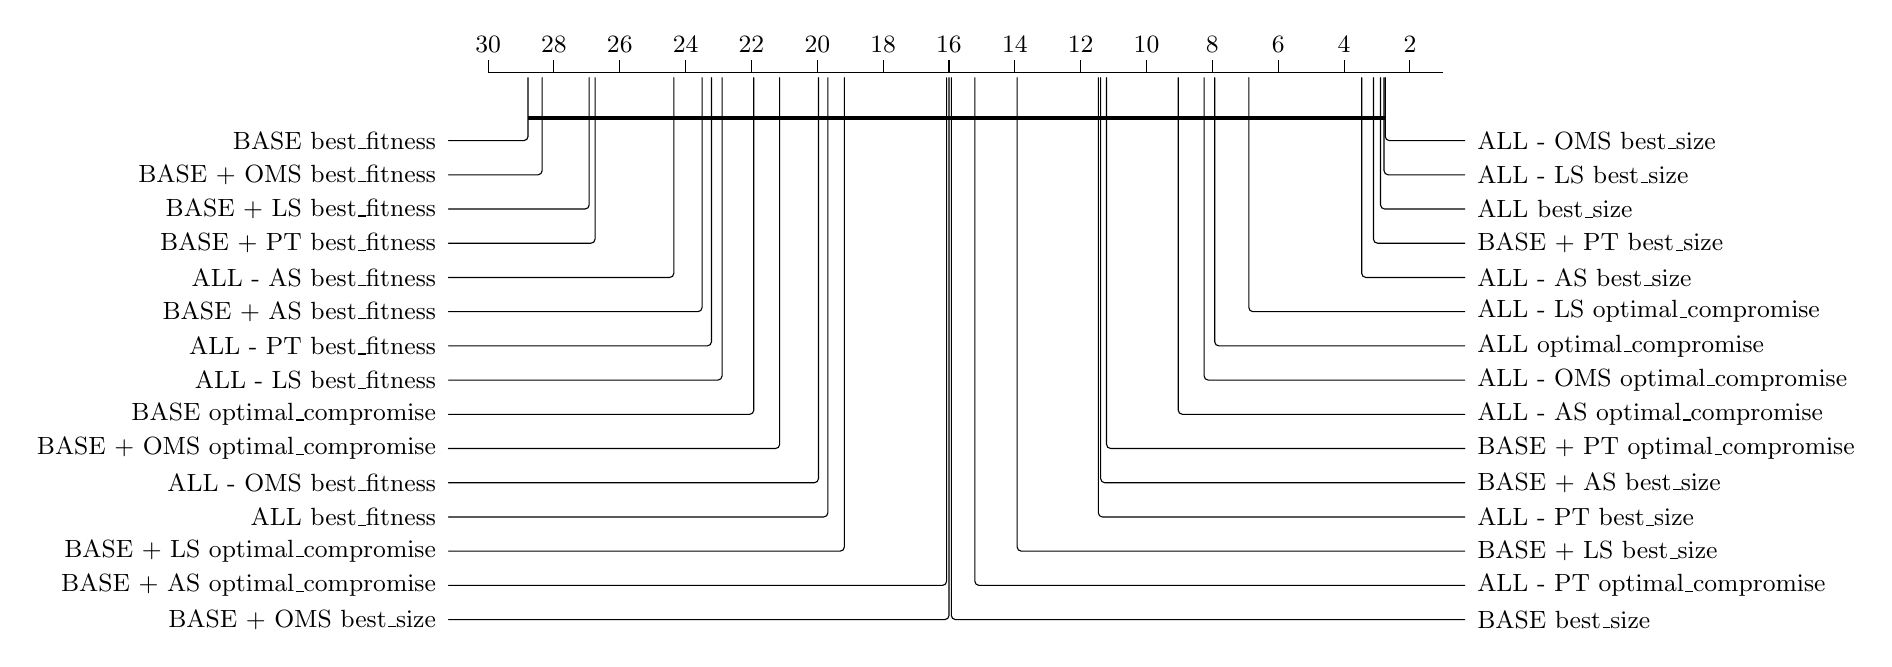
\begin{tikzpicture}[
  treatment line/.style={rounded corners=1.5pt, line cap=round, shorten >=1pt},
  treatment label/.style={font=\small},
  group line/.style={ultra thick},
]

\begin{axis}[
  clip={false},
  axis x line={center},
  axis y line={none},
  axis line style={-},
  xmin={1},
  ymax={0},
  scale only axis={true},
  width={\linewidth},
  ticklabel style={anchor=south, yshift=1.3*\pgfkeysvalueof{/pgfplots/major tick length}, font=\small},
  every tick/.style={draw=black},
  major tick style={yshift=.5*\pgfkeysvalueof{/pgfplots/major tick length}},
  minor tick style={yshift=.5*\pgfkeysvalueof{/pgfplots/minor tick length}},
  title style={yshift=\baselineskip},
  xmax={30},
  ymin={-16.5},
  height={17\baselineskip},
  x dir={reverse},
]

\draw[treatment line] ([yshift=-2pt] axis cs:2.75, 0) |- (axis cs:0.25, -2.0)
  node[treatment label, anchor=west] {ALL - OMS best\_size};
\draw[treatment line] ([yshift=-2pt] axis cs:2.7857142857142856, 0) |- (axis cs:0.25, -3.0)
  node[treatment label, anchor=west] {ALL - LS best\_size};
\draw[treatment line] ([yshift=-2pt] axis cs:2.892857142857143, 0) |- (axis cs:0.25, -4.0)
  node[treatment label, anchor=west] {ALL best\_size};
\draw[treatment line] ([yshift=-2pt] axis cs:3.107142857142857, 0) |- (axis cs:0.25, -5.0)
  node[treatment label, anchor=west] {BASE + PT best\_size};
\draw[treatment line] ([yshift=-2pt] axis cs:3.4642857142857144, 0) |- (axis cs:0.25, -6.0)
  node[treatment label, anchor=west] {ALL - AS best\_size};
\draw[treatment line] ([yshift=-2pt] axis cs:6.892857142857143, 0) |- (axis cs:0.25, -7.0)
  node[treatment label, anchor=west] {ALL - LS optimal\_compromise};
\draw[treatment line] ([yshift=-2pt] axis cs:7.928571428571429, 0) |- (axis cs:0.25, -8.0)
  node[treatment label, anchor=west] {ALL optimal\_compromise};
\draw[treatment line] ([yshift=-2pt] axis cs:8.25, 0) |- (axis cs:0.25, -9.0)
  node[treatment label, anchor=west] {ALL - OMS optimal\_compromise};
\draw[treatment line] ([yshift=-2pt] axis cs:9.035714285714286, 0) |- (axis cs:0.25, -10.0)
  node[treatment label, anchor=west] {ALL - AS optimal\_compromise};
\draw[treatment line] ([yshift=-2pt] axis cs:11.214285714285714, 0) |- (axis cs:0.25, -11.0)
  node[treatment label, anchor=west] {BASE + PT optimal\_compromise};
\draw[treatment line] ([yshift=-2pt] axis cs:11.392857142857142, 0) |- (axis cs:0.25, -12.0)
  node[treatment label, anchor=west] {BASE + AS best\_size};
\draw[treatment line] ([yshift=-2pt] axis cs:11.464285714285714, 0) |- (axis cs:0.25, -13.0)
  node[treatment label, anchor=west] {ALL - PT best\_size};
\draw[treatment line] ([yshift=-2pt] axis cs:13.928571428571429, 0) |- (axis cs:0.25, -14.0)
  node[treatment label, anchor=west] {BASE + LS best\_size};
\draw[treatment line] ([yshift=-2pt] axis cs:15.214285714285714, 0) |- (axis cs:0.25, -15.0)
  node[treatment label, anchor=west] {ALL - PT optimal\_compromise};
\draw[treatment line] ([yshift=-2pt] axis cs:15.928571428571429, 0) |- (axis cs:0.25, -16.0)
  node[treatment label, anchor=west] {BASE best\_size};
\draw[treatment line] ([yshift=-2pt] axis cs:16.0, 0) |- (axis cs:31.285714285714285, -16.0)
  node[treatment label, anchor=east] {BASE + OMS best\_size};
\draw[treatment line] ([yshift=-2pt] axis cs:16.071428571428573, 0) |- (axis cs:31.285714285714285, -15.0)
  node[treatment label, anchor=east] {BASE + AS optimal\_compromise};
\draw[treatment line] ([yshift=-2pt] axis cs:19.178571428571427, 0) |- (axis cs:31.285714285714285, -14.0)
  node[treatment label, anchor=east] {BASE + LS optimal\_compromise};
\draw[treatment line] ([yshift=-2pt] axis cs:19.678571428571427, 0) |- (axis cs:31.285714285714285, -13.0)
  node[treatment label, anchor=east] {ALL best\_fitness};
\draw[treatment line] ([yshift=-2pt] axis cs:19.964285714285715, 0) |- (axis cs:31.285714285714285, -12.0)
  node[treatment label, anchor=east] {ALL - OMS best\_fitness};
\draw[treatment line] ([yshift=-2pt] axis cs:21.142857142857142, 0) |- (axis cs:31.285714285714285, -11.0)
  node[treatment label, anchor=east] {BASE + OMS optimal\_compromise};
\draw[treatment line] ([yshift=-2pt] axis cs:21.928571428571427, 0) |- (axis cs:31.285714285714285, -10.0)
  node[treatment label, anchor=east] {BASE optimal\_compromise};
\draw[treatment line] ([yshift=-2pt] axis cs:22.892857142857142, 0) |- (axis cs:31.285714285714285, -9.0)
  node[treatment label, anchor=east] {ALL - LS best\_fitness};
\draw[treatment line] ([yshift=-2pt] axis cs:23.214285714285715, 0) |- (axis cs:31.285714285714285, -8.0)
  node[treatment label, anchor=east] {ALL - PT best\_fitness};
\draw[treatment line] ([yshift=-2pt] axis cs:23.5, 0) |- (axis cs:31.285714285714285, -7.0)
  node[treatment label, anchor=east] {BASE + AS best\_fitness};
\draw[treatment line] ([yshift=-2pt] axis cs:24.357142857142858, 0) |- (axis cs:31.285714285714285, -6.0)
  node[treatment label, anchor=east] {ALL - AS best\_fitness};
\draw[treatment line] ([yshift=-2pt] axis cs:26.75, 0) |- (axis cs:31.285714285714285, -5.0)
  node[treatment label, anchor=east] {BASE + PT best\_fitness};
\draw[treatment line] ([yshift=-2pt] axis cs:26.928571428571427, 0) |- (axis cs:31.285714285714285, -4.0)
  node[treatment label, anchor=east] {BASE + LS best\_fitness};
\draw[treatment line] ([yshift=-2pt] axis cs:28.357142857142858, 0) |- (axis cs:31.285714285714285, -3.0)
  node[treatment label, anchor=east] {BASE + OMS best\_fitness};
\draw[treatment line] ([yshift=-2pt] axis cs:28.785714285714285, 0) |- (axis cs:31.285714285714285, -2.0)
  node[treatment label, anchor=east] {BASE best\_fitness};
\draw[group line] (axis cs:2.75, -1.3333333333333333) -- (axis cs:28.785714285714285, -1.3333333333333333);

\end{axis}
\end{tikzpicture}